\subsection{XOR}

XOR - это побитовое сложение по модулю (с инвертированием при переполнении), 
например, $1+1=0$ т.к. $1$ - максимальное значение. Все варианты:

$$0 \oplus 0=0$$
$$0 \oplus 1=1$$
$$1 \oplus 1=0$$

\subsubsection{Описание}
То есть, операция $z = x \oplus y$ по сути поразрядная (побитовая — 
результат не зависит от соседних битов). Если только один из 
соответствующих битов равен 1, то результат 1. А если оба 0 или 
оба 1, то результат 0. Если внимательно посмотреть на результат 
применения XOR к двум двоичным числам, то можно заметить, что 
мы можем восстановить одно из слагаемых при помощи второго: $x 
= z \oplus y$ или $y = z \oplus x$. 

\subsubsection{Криптоанализ}

Отсюда можно сделать следующие выводы: зная число y и применяя 
XOR к $x$, мы получим $z$. Затем, мы, опять же используя $y$, получим 
из $z$ обратно число $x$. Таким образом мы можем преобразовать последовательность 
чисел $(x)_i$ в последовательность $(z)_i$. Теперь мы можем назвать 
число y кодирующим (или шифрующим) ключом. Если человек не знает 
ключа, то он не сможет восстановить исходную последовательность 
чисел $(x)_i$.

Поскольку каждая буква будет представлена в шифротексте 
одним и тем же кодом $z$, то воспользуясь частотным словарем взломщик 
сможет вычислить шифрующий ключ $y$, если у него будет в распряжениии 
достаточно длинный шифротекст. 

В случае длинного ключа применяются уже разодранные методы 
анализа из шифра Виженера.

\begin{figure}[H]
\noindent\centering{
    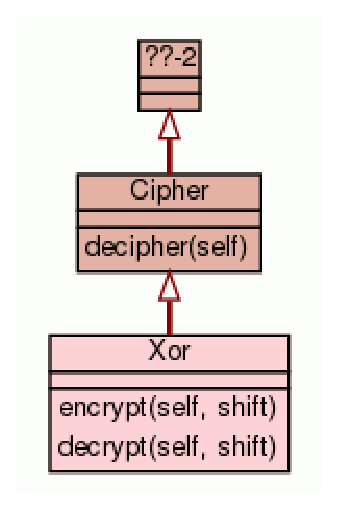
\includegraphics[width=35mm]{\globalImages/uml_xor.eps}
}
\caption{UML диаграмма класса анализа шифра XOR}
\label{figXOR}
\end{figure}
